\documentclass[../main.tex]{subfiles}

\pagestyle{main}
\renewcommand{\chaptermark}[1]{\markboth{\chaptername\ \thechapter: #1}{}}
\setcounter{chapter}{5}

\begin{document}




\chapter{Inner Product Spaces}
\section{Inner Products and Norms}
\begin{itemize}
    \item \marginnote{9/30:}\textbf{Norm} (of $x\in\R^n$): The length of $x$. \emph{Denoted by} $\norm{x}$. \emph{Given by}
    \begin{equation*}
        \norm{x} = \sqrt{x_1^2+\cdots+x_n^2}
    \end{equation*}
    \item \textbf{Dot product} (of $x,y\in\R^n$): The quantity
    \begin{equation*}
        x\cdot y = x_1y_1+\cdots+x_ny_n
    \end{equation*}
    \item Properties of the dot product:
    \begin{itemize}
        \item $x\cdot x=\norm{x}^2$.
        \item $x\cdot x\geq 0$.
        \item $x\cdot x=0$ iff $x=0$.
        \item Let $y\in\R^n$. Then $T:\R^n\to\R$ defined by $Tx=x\cdot y$ is linear.
        \item $x\cdot y=y\cdot x$.
    \end{itemize}
    \item \textbf{Norm} (of $z\in\C^n$): The quantity
    \begin{equation*}
        \norm{z} = \sqrt{|z_1|^2+\cdots+|z_n|^2}
    \end{equation*}
    \begin{itemize}
        \item Note that $\norm{z}^2=z\cdot\bar{z}$.
    \end{itemize}
    \item \textbf{Inner product} (on $V$): A function that takes each ordered pair $(u,v)\in V$ to a number $\inp{u}{v}\in\F$ and has the following properties.
    \begin{description}
        \item[positivity] \hfill\\ $\inp{v}{v}\geq 0$ for all $v\in V$.
        \item[definiteness] \hfill\\ $\inp{v}{v}=0$ iff $v=0$.
        \item[additivity in first slot] \hfill\\ $\inp{u+v}{v}=\inp{u}{w}+\inp{v}{w}$ for all $u,v,w\in V$.
        \item[homogeneity in first slot] \hfill\\ $\inp{\lambda u}{v}=\lambda\inp{u}{v}$ for all $\lambda\in\F$ and all $u,v\in V$.
        \item[conjugate symmetry] \hfill\\ $\inp{u}{v}=\overline{\inp{v}{u}}$ for all $u,v\in V$.
    \end{description}
    \begin{itemize}
        \item Since every real number equals its complex conjugate, if $V$ is real, we can dispense with the conjugacy condition in the conjugate symmetry condition and just have $\inp{u}{v}=\inp{v}{u}$.
        \item \dq{Although most mathematicians define an inner product as above, many physicists use a definition that requires homogeneity in the second slot instead of the first}{166}
    \end{itemize}
    \item \textbf{Euclidean inner product} (on $\F^n$): The function defined by
    \begin{equation*}
        \inp{w}{z} = w_1\bar{z_1}+\cdots+w_n\bar{z_n}
    \end{equation*}
    \item \textbf{Inner product space}: A vector space $V$ along with an inner product on $V$.
    \begin{itemize}
        \item When $\F^n$ is referred to as an inner product space, assume that the inner product is the Euclidean inner product unless explicitly stated otherwise.
    \end{itemize}
    \item Basic properties of an inner product.
    \begin{theorem}\label{trm:inpProperties}\leavevmode
        \begin{enumerate}[label={\textup{(}\alph*\textup{)}},ref={\thetheorem\arabic*}]
            \item \label{trm:inpPropertiesa}For each fixed $u\in V$, the function that takes $v$ to $\inp{v}{u}$ is a linear map from $V$ to $\F$.
            \begin{proof}
                Let $u\in V$ be arbitrary, and let $T:V\to\F$ be defined by $Tv=\inp{v}{u}$. Let $v,w\in V$ be arbitrary, and let $\lambda\in\F$. Then
                \begin{align*}
                    T(v+w) &= \inp{v+w}{u}&
                        T(\lambda v) &= \inp{\lambda v}{u}\\
                    &= \inp{v}{u}+\inp{w}{u}&
                        &= \lambda\inp{v}{u}\\
                    &= Tv+Tw&
                        &= \lambda Tv
                \end{align*}
                as desired.
            \end{proof}
            \item \label{trm:inpPropertiesb}$\inp{0}{u}=0$ for every $u\in V$.
            \begin{proof}
                Let $u\in V$ be arbitrary. Since $T$ as defined above is linear, Theorem \ref{trm:linSendsZero} implies that $0=T(0)=\inp{0}{u}$, as desired.
            \end{proof}
            \item \label{trm:inpPropertiesc}$\inp{u}{0}=0$ for every $u\in V$.
            \begin{proof}
                Let $u\in V$ be arbitrary. By the conjugate symmetry property and the above, $\inp{u}{0}=\overline{\inp{0}{u}}=\bar{0}=0$, as desired.
            \end{proof}
            \item \label{trm:inpPropertiesd}$\inp{u}{v+w}=\inp{u}{v}+\inp{u}{w}$ for all $u,v,w\in V$.
            \begin{proof}
                Let $u,v,w\in V$ be arbitrary. Then
                \begin{align*}
                    \inp{u}{v+w} &= \overline{\inp{v+w}{u}}\\
                    &= \overline{\inp{v}{u}+\inp{w}{u}}\\
                    &= \overline{\inp{v}{u}}+\overline{\inp{w}{u}}\tag*{Theorem \ref{trm:propertiesComplex}}\\
                    &= \inp{u}{v}+\inp{v}{w}
                \end{align*}
                as desired.
            \end{proof}
            \item \label{trm:inpPropertiese}$\inp{u}{\lambda v}=\bar{\lambda}\inp{u}{v}$ for all $\lambda\in\F$ and $u,v\in V$.
            \begin{proof}
                Let $u,v\in V$, and let $\lambda\in\F$. Then
                \begin{align*}
                    \inp{u}{\lambda v} &= \overline{\inp{\lambda v}{u}}\\
                    &= \overline{\lambda\inp{v}{u}}\\
                    &= \bar{\lambda}\overline{\inp{v}{u}}\tag*{Theorem \ref{trm:propertiesComplex}}\\
                    &= \bar{\lambda}\inp{u}{v}
                \end{align*}
            \end{proof}
        \end{enumerate}
    \end{theorem}
    \item \textbf{Norm} (of $v\in V$): The quantity
    \begin{equation*}
        \norm{v} = \sqrt{\inp{v}{v}}
    \end{equation*}
    \item Basic properties of the norm.
    \begin{theorem}\label{trm:normProperties}
        Suppose $v\in V$. Then
        \begin{enumerate}[label={\textup{(}\alph*\textup{)}},ref={\thetheorem\alph*}]
            \item \label{trm:normPropertiesa}$\norm{v}=0$ iff $v=0$.
            \begin{proof}
                Suppose first that $\norm{v}=0$. Then $0=\sqrt{\inp{v}{v}}=\inp{v}{v}$. Thus, $v=0$. The proof is symmetric in the reverse direction.
            \end{proof}
            \item \label{trm:normPropertiesb}$\norm{\lambda v}=|\lambda|\norm{v}$ for all $\lambda\in\F$.
            \begin{proof}
                Let $\lambda\in\F$ be arbitrary. Then
                \begin{align*}
                    \norm{\lambda v}^2 &= \inp{\lambda v}{\lambda v}\\
                    &= \lambda\bar{\lambda}\inp{v}{v}\\
                    &= |\lambda|^2\norm{v}^2\tag*{Theorem \ref{trm:propertiesComplex}}
                \end{align*}
                Taking square roots of the above gives the desired equality.\footnote{Notice this technique: Working with norms squared is usually easier than working directly with norms.}
            \end{proof}
        \end{enumerate}
    \end{theorem}
    \item \textbf{Orthogonal} (vectors $u,v\in V$): Two vectors $u,v\in V$ such that $\inp{u}{v}=0$.\footnote{The word \emph{orthogonal} derives from the Greek word \emph{orthogonios}, which means right-angled.}
    \item If $u,v\in\R^2$ are nonzero, then $\inp{u}{v}=\norm{u}\norm{v}\cos\theta$.
    \begin{itemize}
        \item \dq{Thus, two vectors in $\R^2$ are orthogonal (with respect to the usual Euclidean inner product) if and only if the cosine of the angle between them is 0, which happens if and only if the vectors are perpendicular in the usual sense of plane geometry. Thus, you can think of the word \emph{orthogonal} as a fancy word meaning \emph{perpendicular}.}{169}
    \end{itemize}
    \item Orthogonality and zero.
    \begin{theorem}\leavevmode
        \begin{enumerate}[label={\textup{(}\alph*\textup{)}}]
            \item $0$ is orthogonal to every vector in $V$.
            \begin{proof}
                Let $u\in V$ be arbitrary. Then Theorem \ref{trm:inpPropertiesb} implies that $\inp{0}{u}=0$. Thus, $u$ and 0 are orthogonal, as desired.
            \end{proof}
            \item $0$ is the only vector in $V$ that is orthogonal to itself.
            \begin{proof}
                Let $v\in V$ be such that $v$ is orthogonal to itself. Then $\inp{v}{v}=0$. But by the property of definiteness, it follows that $v=0$, as desired.
            \end{proof}
        \end{enumerate}
    \end{theorem}
    \item The special case where $V=\R^2$ of the following is over $\num{2500}$ years old, although the following is not the original proof.
    \begin{theorem}[Pythagorean Theorem]\label{trm:pythagorean}
        Suppose $u,v\in V$ are orthogonal. Then
        \begin{equation*}
            \norm{u+v}^2 = \norm{u}^2+\norm{v}^2
        \end{equation*}
        \begin{proof}
            We have
            \begin{align*}
                \norm{u+v}^2 = \inp{u+v}{u+v}\\
                &= (\inp{u}{u}+\inp{u}{v})+(\inp{v}{u}+\inp{v}{v})\\
                &= \norm{u}^2+0+0+\norm{v}^2\\
                &= \norm{u}^2+\norm{v}^2
            \end{align*}
            as desired.
        \end{proof}
    \end{theorem}
    \begin{itemize}
        \item Note that we can prove the converse of the Pythagorean Theorem in \emph{real} inner product spaces as follows: If $\norm{u+v}^2=\norm{u}^2+\norm{v}^2$ for $u,v$ real, then
        \begin{align*}
            0 &= \inp{u}{v}+\inp{v}{u}\\
            &= \inp{u}{v}+\overline{\inp{u}{v}}\\
            &= 2\Re\inp{u}{v}\\
            &= \inp{u}{v}
        \end{align*}
        as desired.
    \end{itemize}
    \item Let $u,v\in V$ with $v\neq 0$. We are now equipped to consider how to write $u$ as the sum of $v$ plus a vector $w$ orthogonal to $v$, as in Figure \ref{fig:orthogonalDecomposition} below.
    \begin{theorem}\label{trm:orthogonalDecomposition}
        Suppose $u,v\in V$ with $v\neq 0$. Set $c=\frac{\inp{u}{v}}{\norm{v}^2}$ and $w=u-\frac{\inp{u}{v}}{\norm{v}^2}v$. Then $\inp{w}{v}=0$ and $u=cv+w$.
        \begin{figure}[h!]
            \centering
            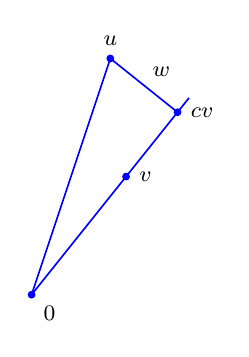
\begin{tikzpicture}[
                every path/.append style={blue,semithick},
                every node/.append style={black}
            ]
                \footnotesize
                \draw (0,0) node[circle,fill=blue,inner sep=1pt,label={below right:$0$}]{} -- (1,3) node[circle,fill=blue,inner sep=1pt,label={above:$u$}]{};
                \draw (0,0) -- node[pos=0.6,circle,fill=blue,inner sep=1pt,label={right:$v$}]{} (2,2.5);
                \draw ({76/41},{95/41}) node[circle,fill=blue,inner sep=1pt,label={right:$cv$}]{} -- node[above right]{$w$} (1,3);
            \end{tikzpicture}
            \caption{An orthogonal decomposition.}
            \label{fig:orthogonalDecomposition}
        \end{figure}
        \begin{proof}
            We want to write $u$ in the form $u=cv+w$ where $w$ is orthogonal to $v$. We know that
            \begin{equation*}
                u=cv+(u-cv)
            \end{equation*}
            so we need only choose $c$ such that $v$ is orthogonal to $u-cv$. In other words, we want
            \begin{align*}
                0 &= \inp{u-cv}{v}\\
                &= \inp{u}{v}+\inp{-cv}{v}\\
                &= \inp{u}{v}-c\inp{v}{v}\\
                &= \inp{u}{v}-c\norm{v}^2\\
                c &= \frac{\inp{u}{v}}{\norm{v}^2}
            \end{align*}
            But this gives the values we want for $c$ and $w$, as desired.
        \end{proof}
    \end{theorem}
    \item This allows for the proof of a very important result.
    \begin{theorem}[Cauchy-Schwarz Inequality]\label{trm:CauchySchwarz}
        Suppose $u,v\in V$. Then
        \begin{equation*}
            |\inp{u}{v}| \leq \norm{u}\norm{v}
        \end{equation*}
        This inequality is an equality if and only if one of $u,v$ is a scalar multiple of the other.
        \begin{proof}
            We divide into two cases ($v=0$ and $v\neq 0$). If $v=0$, then
            \begin{equation*}
                |\inp{u}{v}| = 0 \leq 0 = \norm{u}\sqrt{0} = \norm{u}\sqrt{\inp{u}{v}} = \norm{u}\norm{v}
            \end{equation*}
            and we also have that the equality holds since $v=0=0u$, $0\in\F$. Now let $v\neq 0$. Then by Theorem \ref{trm:orthogonalDecomposition},
            \begin{equation*}
                u = \frac{\inp{u}{v}}{\norm{v}^2}v+w
            \end{equation*}
            where $\inp{v}{w}=0$. It follows by the \hyperref[trm:pythagorean]{Pythagorean Theorem} that
            \begin{align*}
                \norm{u}^2 &= \norm{\frac{\inp{u}{v}}{\norm{v}^2}v}^2+\norm{w}^2\\
                &= \inp{\frac{\inp{u}{v}}{\norm{v}^2}v}{\frac{\inp{u}{v}}{\norm{v}^2}v}+\norm{w}^2\\
                &= \frac{\inp{u}{v}}{\norm{v}^2}\overline{\frac{\inp{u}{v}}{\norm{v}^2}}\inp{v}{v}+\norm{w}^2\\
                &= \frac{\inp{u}{v}\overline{\inp{u}{v}}}{\norm{v}^4}\norm{v}^2+\norm{w}^2\\
                &= \frac{|\inp{u}{v}|^2}{\norm{v}^2}+\norm{w}^2\\
                &\geq \frac{|\inp{u}{v}|^2}{\norm{v}^2}
            \end{align*}
            Multiplying both sides by $\norm{v}^2$ and taking square roots gives the desired inequality.\par
            Also note that the Cauchy-Schwarz inequality is an equality iff the last line is an equality, which happens iff $w=0$. But $w=0$ iff $u$ is a scalar multiple of $v$, as desired.
        \end{proof}
    \end{theorem}
    \item Note that the Cauchy-Schwarz is known as such because the French mathematician Augustin-Louis Cauchy proved the top inequality below in 1821, and the German mathematician Hermann Schwarz proved the bottom inequality below in 1886; both are special cases of the above.
    \begin{gather*}
        |x_1y_1+\cdots+x_ny_n|^2 \leq (x_1^2+\cdots+x_n^2)(y_1^2+\cdots+y_n^2)\\
        \left| \int_{-1}^1f(x)g(x)\dd{x} \right|^2 \leq \left( \int_{-1}^1(f(x))^2\dd{x} \right)\left( \int_{-1}^1(g(x))^2\dd{x} \right)
    \end{gather*}
    \begin{itemize}
        \item For the top one, we let $x_1,\dots,x_n,y_1,\dots,y_n\in\R$.
        \item For the bottom one, we let $f,g$ be continuous real-valued functions on $[-1,1]$.
    \end{itemize}
    \item We now prove another important inequality.
    \begin{theorem}[Triangle Inequality]
        Suppose $u,v\in V$. Then
        \begin{equation*}
            \norm{u+v} \leq \norm{u}+\norm{v}
        \end{equation*}
        This inequality is an equality if and only if one of $u,v$ is a nonnegative multiple of the other.
        \begin{proof}
            We have
            \begin{align*}
                \norm{u+v}^2 &= \inp{u+v}{u+v}\\
                &= \inp{u}{u}+\inp{v}{v}+\inp{u}{v}+\inp{v}{u}\\
                &= \inp{u}{u}+\inp{v}{v}+\inp{u}{v}+\overline{\inp{u}{v}}\\
                &= \norm{u}^2+\norm{v}^2+2\Re\inp{u}{v}\\
                &\leq \norm{u}^2+\norm{v}^2+2|\inp{u}{v}|\\
                &\leq \norm{u}^2+\norm{v}^2+2\norm{u}\norm{v}\tag*{\hyperref[trm:CauchySchwarz]{Cauchy-Schwarz Inequality}}\\
                &= (\norm{u}+\norm{v})^2
            \end{align*}
            Taking square roots of both sides gives the desired inequality.\par
            This inequality is an equality iff $\inp{u}{v}=\norm{u}\norm{v}$. Now suppose $u=cv$ where $c\in\F$ is positive. Then
            \begin{align*}
                \inp{u}{v} &= \inp{cv}{v}\\
                &= c\inp{v}{v}\\
                &= c\norm{v}^2\\
                &= c\sqrt{\inp{v}{v}}\norm{v}\\
                &= \sqrt{c^2\inp{v}{v}}\norm{v}\\
                &= \sqrt{\inp{cv}{cv}}\norm{v}\\
                &= \norm{u}\norm{v}
            \end{align*}
            The proof is the same in the reverse direction.
        \end{proof}
    \end{theorem}
    \item One last equality.
    \begin{theorem}[Parallelogram Equality]
        Suppose $u,v\in V$. Then
        \begin{equation*}
            \norm{u+v}^2+\norm{u-v}^2 = 2(\norm{u}^2+\norm{v}^2 )
        \end{equation*}
        \begin{figure}[h!]
            \centering
            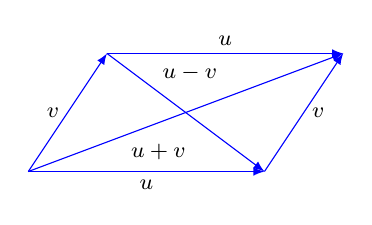
\begin{tikzpicture}[
                every path/.append style={blue,-latex},
                every node/.append style={black}
            ]
                \footnotesize
                \coordinate (a) at (0,0);
                \coordinate (b) at (3,0);
                \coordinate (c) at (4,1.5);
                \coordinate (d) at (1,1.5);

                \draw (a) -- node[below]{$u$} (b);
                \draw (b) -- node[right]{$v$} (c);
                \draw (d) -- node[above]{$u$} (c);
                \draw (a) -- node[left]{$v$}  (d);
                \draw (a) -- node[pos=0.3,below right]{$u+v$} (c);
                \draw (d) -- node[pos=0.3,above right]{$u-v$} (b);
            \end{tikzpicture}
            \caption{The parallelogram equality.}
            \label{fig:parallelogramEquality}
        \end{figure}
        \begin{proof}
            We have
            \begin{align*}
                \norm{u+v}^2+\norm{u-v}^2 &= \inp{u+v}{u+v}+\inp{u-v}{u-v}\\
                &= \norm{u}^2+\norm{v}^2+\inp{u}{v}+\inp{v}{u}+\norm{u}^2+\norm{v}^2-\inp{u}{v}-\inp{v}{u}\\
                &= 2(\norm{u}^2+\norm{v}^2)
            \end{align*}
            as desired.
        \end{proof}
    \end{theorem}
\end{itemize}



\section{Orthonormal Bases}
\begin{itemize}
    \item \marginnote{10/3:}\textbf{Orthonormal} (list of vectors): A list of vectors such that each vector in the list has norm 1 and is orthogonal to all the other vectors in the list.
    \begin{itemize}
        \item In other words, a list $e_1,\dots,e_m$ is orthonormal if
        \begin{equation*}
            \inp{e_j}{e_k} =
            \begin{cases}
                1 & j=k\\
                0 & j\neq k
            \end{cases}
        \end{equation*}
    \end{itemize}
    \item Orthonormal lists are particularly easy to work with.
    \begin{theorem}\label{trm:normOrthoLnlComb}
        If $e_1,\dots,e_m$ is an orthonormal list of vectors in $V$, then
        \begin{equation*}
            \norm{a_1e_1+\cdots+a_me_m}^2 = |a_1|^2+\cdots+|a_m|^2
        \end{equation*}
        for all $a_1,\dots,a_m\in\F$.
        \begin{proof}
            We have that
            \begin{align*}
                \norm{a_1e_1+\cdots+a_me_m}^2 &= \norm{a_1e_1}^2+\cdots+\norm{a_me_m}^2\tag*{\hyperref[trm:pythagorean]{Pythagorean Theorem}}\\
                &= |a_1|^2\norm{e_1}^2+\cdots+|a_m|^2\norm{e_m}^2\tag*{Theorem \ref{trm:normPropertiesb}}\\
                &= |a_1|^2+\cdots+|a_m|^2
            \end{align*}
            as desired.
        \end{proof}
    \end{theorem}
    \item The next result directly follows from the previous one.
    \begin{theorem}\label{trm:orthonormalLnlIndep}
        Every orthonormal list of vectors is linearly independent.
        \begin{proof}
            Let $e_1,\dots,e_m$ be an orthonormal list of vectors, and let $a_1,\dots,a_m\in\F$ be such that $a_1e_1+\cdots+a_me_m=0$. Then
            \begin{align*}
                0 &= \norm{0}\\
                &= \norm{a_1e_1+\cdots+a_me_m}\\
                &= |a_1|^2+\cdots+|a_m|^2\tag*{Theorem \ref{trm:normOrthoLnlComb}}
            \end{align*}
            But this implies that each $a_j=0$, as desired.
        \end{proof}
    \end{theorem}
    \item \textbf{Orthonormal basis} (of $V$): An orthonormal list of vectors in $V$ that is also a basis of $V$.
    \item We now prove an easy condition for identifying orthonormal bases.
    \begin{theorem}
        Every orthonormal list of vectors in $V$ with length $\dim V$ is an orthonormal basis of $V$.
        \begin{proof}
            Let $e_1,\dots,e_m$ be an orthonormal list of vectors in $V$ with length $\dim V$. It follows by Theorem \ref{trm:orthonormalLnlIndep} that $e_1,\dots,e_m$ is linearly independent. Therefore, by Theorem \ref{trm:sameDimIndependent}, $e_1,\dots,e_m$ is a basis of $V$.
        \end{proof}
    \end{theorem}
\end{itemize}




\end{document}